\documentclass[10pt,a4paper]{article}
\usepackage[left=1.8cm,right=1.8cm,top=1.6cm,bottom=1.75cm]{geometry}
\usepackage[default]{sourcesanspro}
\usepackage{microtype,graphicx,booktabs,amsmath,xcolor,enumitem,fancyhdr}
\usepackage[hidelinks]{hyperref}
\definecolor{accent}{HTML}{DC3522}\definecolor{dark}{HTML}{333333}\definecolor{muted}{HTML}{666666}
\color{dark}\setlength{\parindent}{0pt}\setlength{\parskip}{5pt}
\setlist{nosep,leftmargin=1.4em}\pagestyle{fancy}\fancyhf{}
\fancyfoot[L]{\footnotesize\color{muted}Dr Jesus Ocariz}
\fancyfoot[C]{\footnotesize\color{muted}Exploring GFlowNets for Analog EDA}
\fancyfoot[R]{\footnotesize\color{muted}\thepage}\renewcommand{\headrulewidth}{0pt}
\newcommand{\rsection}[1]{\vspace{4pt}{\large\bfseries\textcolor{accent}{#1}}\par\vspace{-2pt}\textcolor{muted}{\rule{\textwidth}{0.5pt}}}
\begin{document}

{\fontsize{25}{29}\selectfont\bfseries Exploring GFlowNets for Analog EDA}\par
{\large\color{accent}A first mathematical and computational study of diverse Pareto search}\par
\vspace{5pt}{\color{muted}Technical project report \hfill Dr Jesus Ocariz \hfill 12 August 2026}

\rsection{Motivation}

My background is in mathematics and scientific machine learning rather than circuit design. I completed a PhD in Mathematics on nonlinear partial differential equations and geometric analysis, followed by master's-level work in applied mathematics, computer engineering and data science. My data-science thesis and subsequent R\&D work at Sony Europe focused on multi-objective Generative Flow Networks (GFlowNets). This project is my attempt to learn the fundamentals of analog electronic design automation (EDA) through a concrete, reproducible experiment and to ask where that GFlowNet expertise could be useful.

GFlowNets are attractive when the goal is not one optimum but a distribution of diverse, high-reward structured objects. That idea has been explored in molecular and drug discovery, where many chemically distinct candidates may be valuable, and in Neural Architecture Search (NAS), where multiple architectures can occupy different points on an accuracy--complexity frontier [1--3]. Analog design appears to have a related mathematical structure: circuit evaluation is expensive, variables interact nonlinearly, feasibility matters, and designers often need several compromises among gain, speed, power, area and robustness.

I therefore treat EDA as a new application domain, not as something this small experiment has solved. The aim is to test a narrow hypothesis with honest baselines:

\begin{quote}
Can a GFlowNet contribute useful diverse-search behaviour to a multi-objective analog design loop, either as a standalone sampler or as a learned mutation operator inside NSGA-II?
\end{quote}

\rsection{Circuit and design problem}

I chose a resistively loaded common-source NMOS (N-type Metal-Oxide-Semiconductor) amplifier because it is simple enough to understand and simulate quickly, but still exhibits meaningful trade-offs. Six variables each take five discrete values, giving $5^6=15{,}625$ configurations.

\begin{center}\small
\begin{tabular}{lll}\toprule
Variable & Values & Main effect represented \\\midrule
$W$ ($\mu$m) & 2, 4, 8, 16, 32 & Transconductance, capacitance, area \\
$L$ ($\mu$m) & 0.18, 0.27, 0.36, 0.54, 0.72 & Output resistance, speed, area \\
Bias target ($\mu$A) & 20, 40, 80, 160, 320 & Gain, bandwidth, power \\
$R_D$ (k$\Omega$) & 2, 4, 8, 16, 32 & Gain, output pole, headroom \\
$C_L$ (pF) & 0.2, 0.5, 1, 2, 5 & Bandwidth and area proxy \\
$V_{DD}$ (V) & 1.2, 1.5, 1.8, 2.1, 2.5 & Headroom and power \\\bottomrule
\end{tabular}\end{center}

For each selected configuration, ngspice 47 performs an operating-point analysis and an AC sweep from 10 Hz to 10 GHz. The simulation returns low-frequency voltage gain, $-3$ dB bandwidth, DC power and an operating-validity flag. Invalid designs cannot enter the Pareto archive. Results are cached by the six integer design indices, so repeated configurations never consume another simulation.

The MOSFET (Metal-Oxide-Semiconductor Field-Effect Transistor) is represented by a portable Level-1 model. This makes the search pipeline easy to reproduce without proprietary technology data, but it is deliberately modest: the numerical values should not be interpreted as predictions for fabricated silicon.

\rsection{Data and objective space}

The data are generated by the simulator, not taken from a pre-existing database. A scrambled Sobol sequence fixes a 1,024-configuration reference set before method comparison. It defines stable normalisation ranges and an estimated reference front. Each optimisation run then starts with 24 observations and adds six batches of 12, for a total budget of 96 ngspice evaluations.

The four objectives are written in minimisation form,
\[
f(x)=(-G(x),-B(x),P(x),A_{\mathrm{proxy}}(x)),\qquad
A_{\mathrm{proxy}}=WL+0.20R_D+1.50C_L.
\]
Here $G$ is gain, $B$ is bandwidth and $P$ is power. The final term is a transparent technology-independent proxy used to introduce an area trade-off; it is not physical post-layout area.

\begin{figure}[ht]\centering
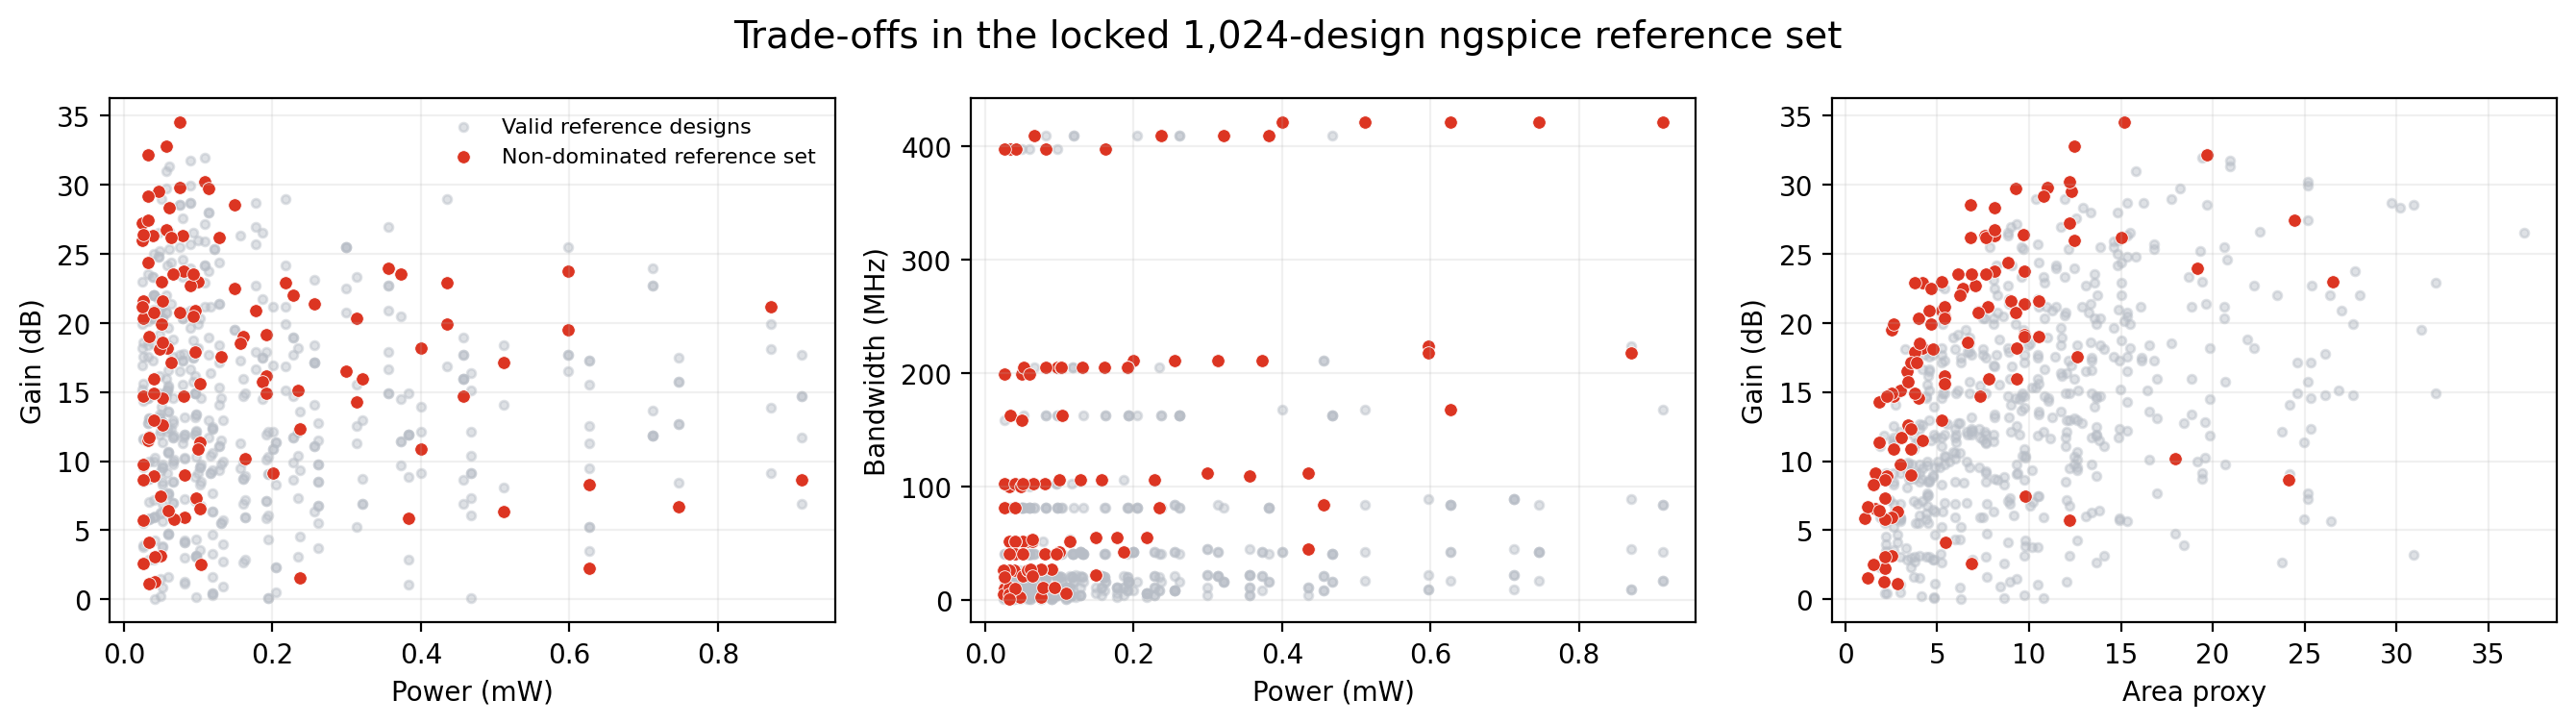
\includegraphics[width=\textwidth]{results/advanced_pareto_ngspice/reference_tradeoffs.png}
\caption{Projections of the locked 1,024-design reference set. Red points are non-dominated in the complete four-dimensional objective space.}
\end{figure}

\rsection{Methods compared}

All adaptive methods use the same seven-model Extra Trees surrogate ensemble. Random Chebyshev preferences expose different parts of the front, while uncertainty and predicted operating validity contribute to acquisition.

\begin{description}[style=nextline]
\item[Random and Sobol] Uniform and low-discrepancy space-filling baselines.
\item[Preference scalarisation] Diverse greedy selection across 64 random objective preferences.
\item[Categorical reward] Direct weighted sampling from exactly the same positive terminal reward used by the standalone GFlowNet. This tests whether performance comes from the reward rather than flow learning.
\item[Surrogate NSGA-II] Non-dominated sorting, crowding distance, tournament selection, crossover and discrete mutation operate on surrogate predictions, following the main components of NSGA-II [4]. Only the selected batch is evaluated with ngspice.
\item[Standalone Pareto GFlowNet] A Trajectory-Balance policy [5] sequentially assigns the six variables. It is updated for 250 steps per acquisition round and samples terminal designs in proportion to the multi-objective acquisition reward.
\item[GFlowNet--NSGA-II feedback] This is the main proposed method. The GFlowNet persists between rounds. Designs that have been evaluated by ngspice and remain non-dominated receive an explicit reward boost. High-reward GFlowNet samples then act as a third parent---an informed mutation donor---inside NSGA-II. The selected offspring are evaluated by ngspice, successful designs update the archive, and that archive trains the GFlowNet in the next round.
\end{description}

The last method creates a feedback loop: NSGA-II contributes selection pressure and local evolutionary search; the GFlowNet learns a reusable distribution from successful designs; and its samples propose structured mutations rather than independent random gene changes.

\rsection{Evaluation}

Hypervolume measures how much of the normalised reference box is dominated by the discovered archive; higher is better. It is estimated with 100,000 fixed common Monte Carlo points. Inverted Generational Distance (IGD) measures distance from the estimated reference front to the discovered set; lower is better. Archive size counts non-dominated designs. Objective spacing is the standard deviation of nearest-neighbour distances on the normalised front, so lower values indicate more uniform coverage.

Every method uses the same five seeds, initial budget, batch sizes, reference set and ngspice cache. Reported values are mean $\pm$ sample standard deviation at 96 evaluations.
\newpage
\rsection{Results}

\begin{center}\scriptsize
\begin{tabular}{lrrrr}\toprule
Method & Hypervolume $\uparrow$ & IGD $\downarrow$ & Non-dominated $\uparrow$ & Spacing $\downarrow$ \\\midrule
GFlowNet--NSGA-II & \textbf{0.526 $\pm$ 0.046} & \textbf{0.161 $\pm$ 0.008} & 32.6 $\pm$ 4.3 & 0.131 $\pm$ 0.013 \\
Surrogate NSGA-II & 0.520 $\pm$ 0.053 & 0.164 $\pm$ 0.016 & 33.0 $\pm$ 1.9 & 0.138 $\pm$ 0.024 \\
Scalarisation & 0.461 $\pm$ 0.032 & 0.175 $\pm$ 0.007 & 37.2 $\pm$ 5.5 & 0.108 $\pm$ 0.043 \\
Categorical reward & 0.410 $\pm$ 0.056 & 0.179 $\pm$ 0.017 & 39.4 $\pm$ 4.7 & 0.110 $\pm$ 0.035 \\
Pareto GFlowNet & 0.401 $\pm$ 0.045 & 0.178 $\pm$ 0.013 & \textbf{41.6 $\pm$ 4.3} & \textbf{0.097 $\pm$ 0.026} \\
Sobol & 0.370 $\pm$ 0.048 & 0.184 $\pm$ 0.011 & 28.0 $\pm$ 1.0 & 0.124 $\pm$ 0.025 \\
Random & 0.290 $\pm$ 0.067 & 0.197 $\pm$ 0.016 & 27.4 $\pm$ 3.0 & 0.139 $\pm$ 0.022 \\\bottomrule
\end{tabular}\end{center}

\begin{figure}[ht]\centering
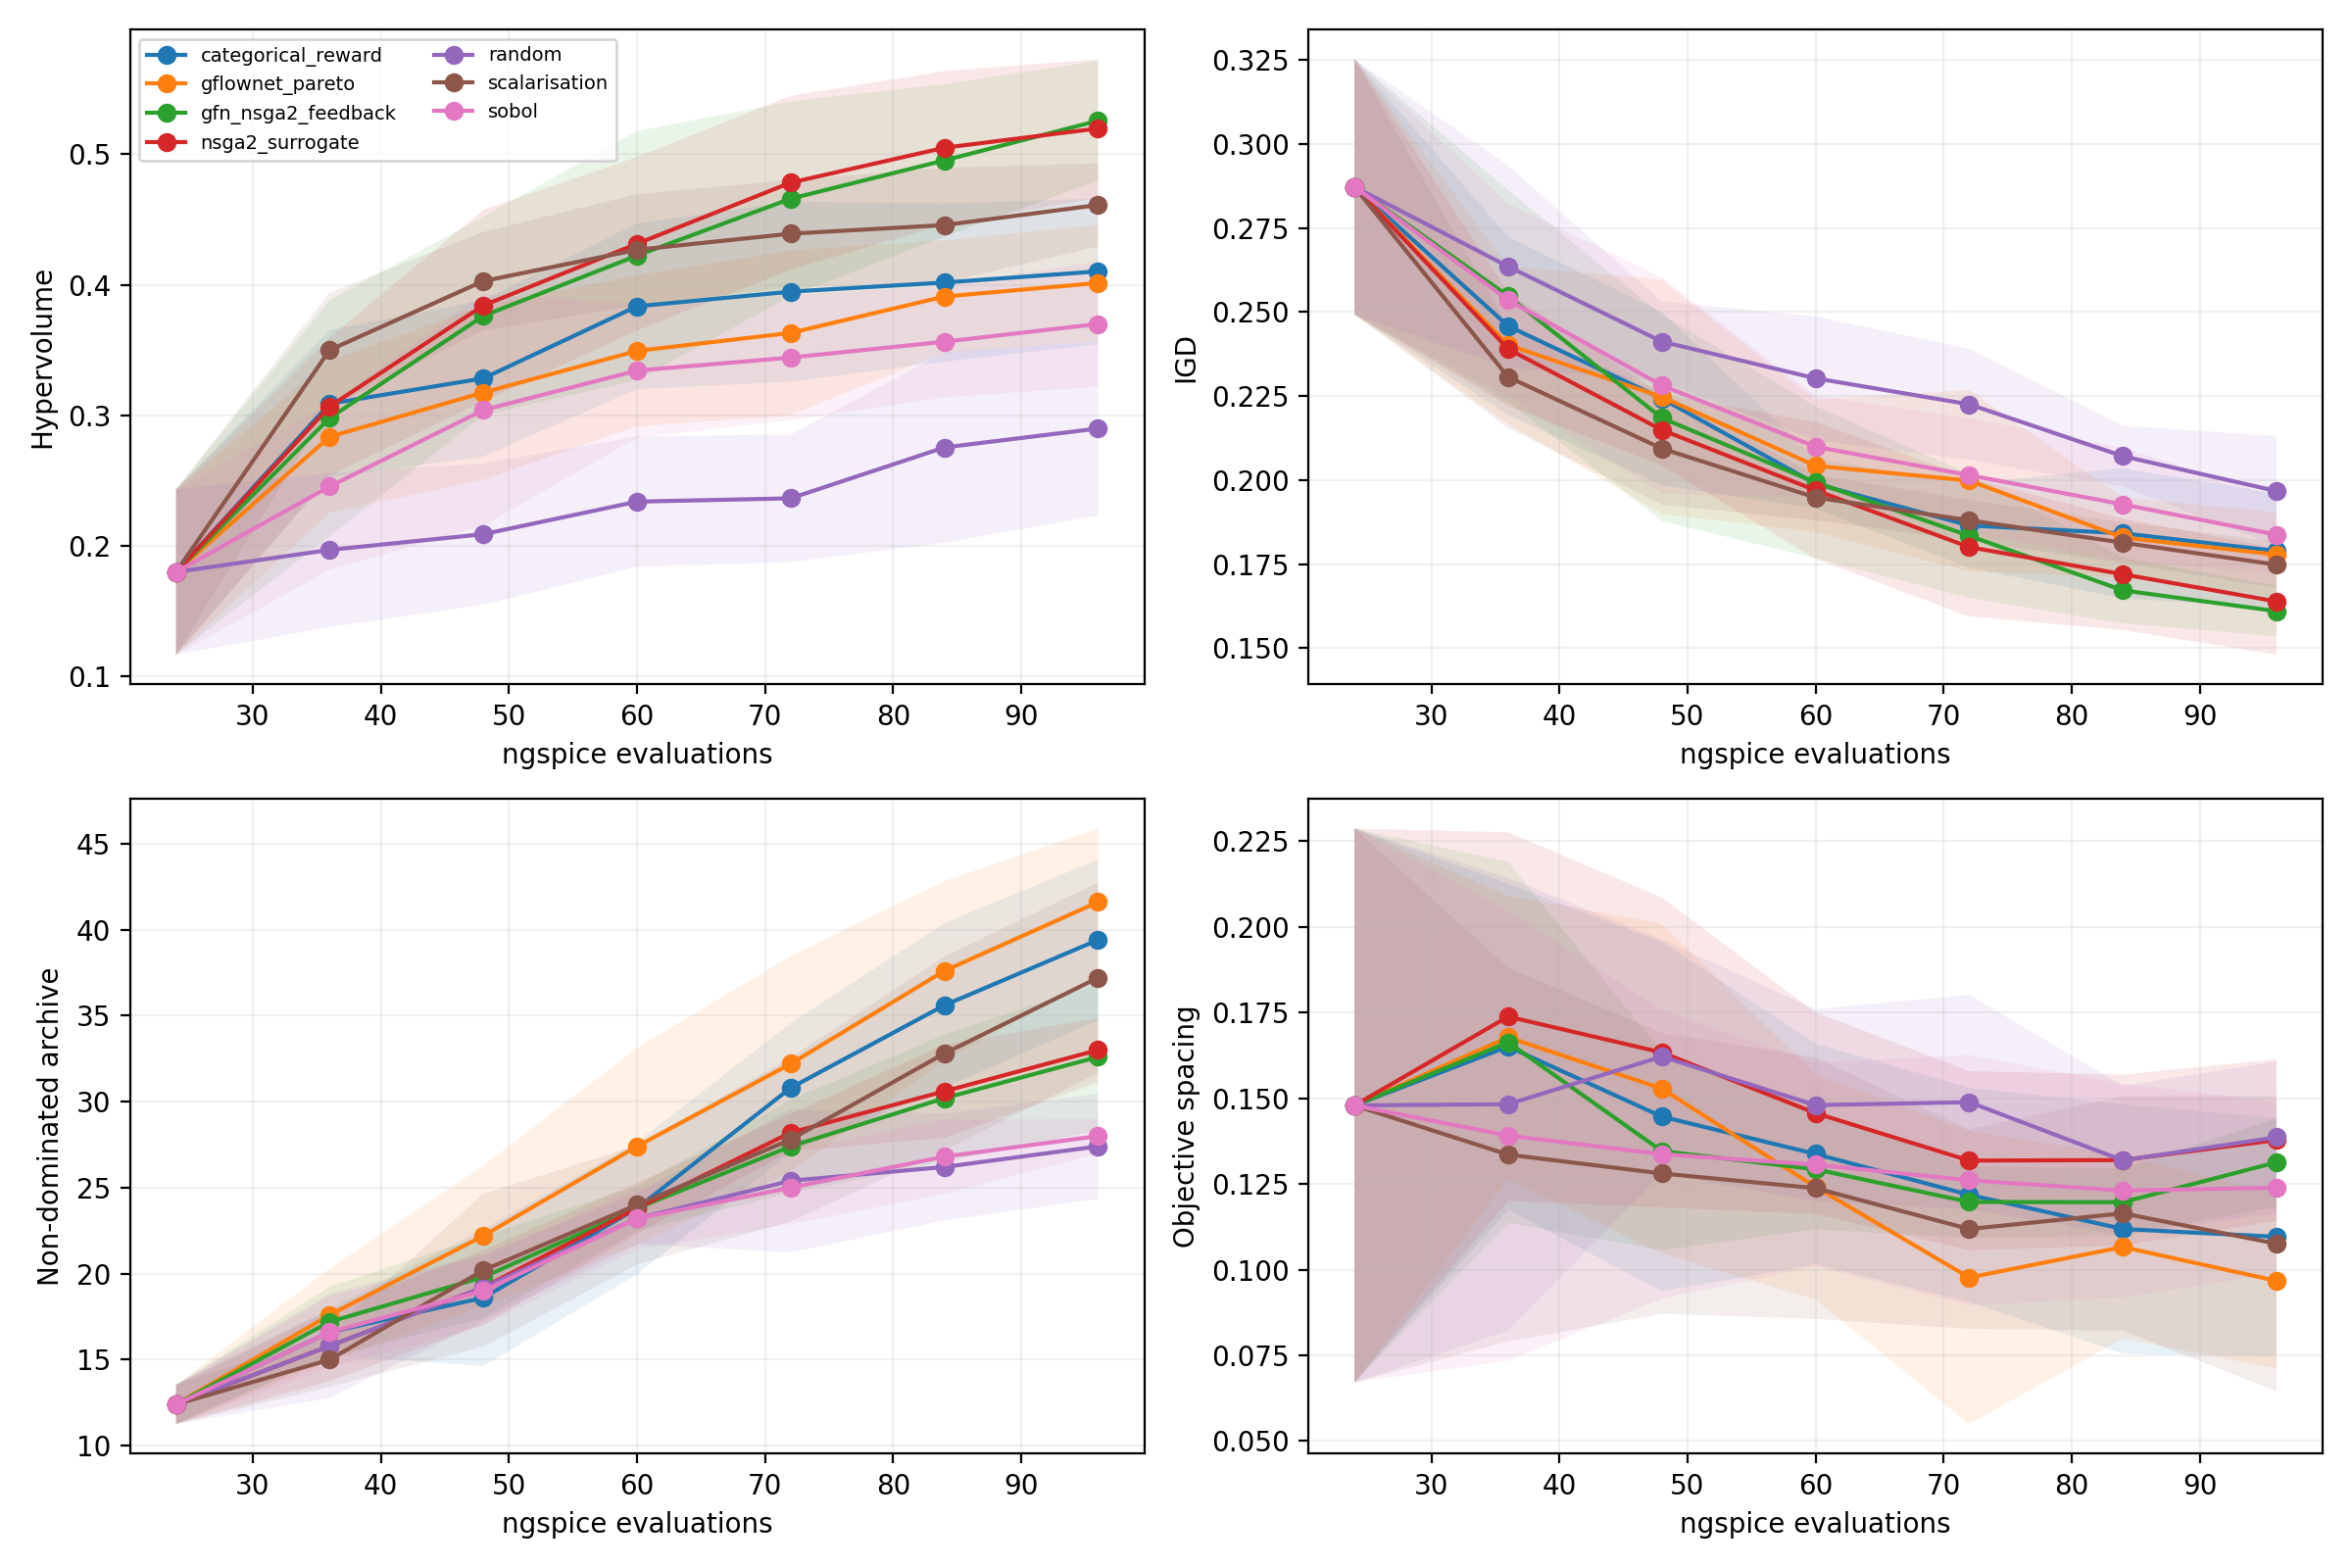
\includegraphics[width=.90\textwidth]{results/advanced_pareto_ngspice/advanced_curves.png}
\caption{Pareto metrics versus ngspice-call budget. Shading represents one sample standard deviation across five seeds.}
\end{figure}

The feedback hybrid has the best mean hypervolume and IGD, improving on NSGA-II by 0.006 and 0.003 respectively. This is encouraging, but seed-level differences change sign. Paired Wilcoxon tests give $p=0.8125$ for hypervolume and $p=1.0$ for IGD. With five seeds, I therefore regard the hybrid as competitive with NSGA-II, not proven superior.

The standalone GFlowNet shows a different strength. It produces the largest non-dominated archive and the lowest spacing statistic, suggesting more numerous and uniformly distributed trade-offs. However, direct categorical sampling from the same reward attains slightly higher hypervolume. The present experiment therefore does not show that flow learning alone improves terminal Pareto quality.

\rsection{What I learned and next steps}

The experiment suggests that GFlowNets may be more useful as a component of an EDA optimiser than as a replacement. NSGA-II provides strong convergence and diversity mechanisms; the GFlowNet can learn reusable structured mutations from successful simulations. The hybrid method should be analised with a larger study.


% \rsection{Reproducibility}

% The experiment requires Python 3.12, ngspice 47 and the packages listed in \texttt{requirements.txt}. From the project directory:
% \begin{verbatim}
% python3 -m pip install -r requirements.txt
% python3 -m pytest -q
% python3 advanced_pareto_experiment.py --backend ngspice \
%   --reference-size 1024 --seeds 0 1 2 3 4 --rounds 6 \
%   --batch-size 12 --gfn-steps 250 --diversity-weight 0.3
% python3 report_plots.py
% xelatex GFlowNet_Analog_EDA_Report_v2.tex
% \end{verbatim}

% The files required to reproduce the study are:

% \begin{itemize}
% \item \texttt{advanced\_pareto\_experiment.py}: all seven methods, feedback loop, locked protocol, statistics and main plots;
% \item \texttt{spice\_simulator.py}: ngspice netlist generation, output parsing and persistent cache interface;
% \item \texttt{simulator.py}: discrete design grid, decoding and compact development oracle;
% \item \texttt{pareto\_experiment.py}: objective construction, dominance, normalisation, hypervolume and IGD;
% \item \texttt{experiment.py}: shared surrogate, GFlowNet, sampling, Sobol and diversity utilities;
% \item \texttt{report\_plots.py}: reference-set visualisation;
% \item \texttt{test\_simulator.py}, \texttt{test\_pareto.py}, and \texttt{test\_advanced\_pareto.py}: nine automated tests;
% \item \texttt{requirements.txt}: Python dependencies.
% \end{itemize}

% Generated outputs are written to \texttt{results/advanced\_pareto\_ngspice}. The optional \texttt{results/ngspice\_cache.json} accelerates reruns but is not required: deleting it forces all circuit evaluations to be regenerated.

\rsection{Selected references}

\small
{[1]} Y. Bengio et al., \emph{GFlowNet Foundations}, 2021. \href{https://arxiv.org/abs/2111.09266}{arXiv:2111.09266}.\par
{[2]} A. C. Nica et al., \emph{Evaluating Generalization in GFlowNets for Molecule Design}, MLDD at ICLR 2022.\par
{[3]} D. Soin et al., \emph{Order-Preserving GFlowNets}, 2024; experiments include molecule generation, multi-objective Pareto approximation and neural architecture search. \href{https://openreview.net/forum?id=VXDPXuq4oG}{OpenReview}.\par
{[4]} K. Deb et al., \emph{A Fast and Elitist Multiobjective Genetic Algorithm: NSGA-II}, IEEE Transactions on Evolutionary Computation, 2002.\par
{[5]} N. Malkin et al., \emph{Trajectory Balance: Improved Credit Assignment in GFlowNets}, NeurIPS 2022. \href{https://openreview.net/forum?id=5btWTw1vcw1}{OpenReview}.

\end{document}
